\documentclass{openevreport}

\renewcommand{\bibname}{References}
\foottext{Version 1.1, 2000-06-19 \newline\scriptsize
Use and duplication of this document or any information
contained herein is subject to the notice on the front of this
document.}

\begin{document}

\begin{titlepage}
\pagestyle{empty}
\centering
\vspace*{0.75in}


\includegraphics[width=2.5in]{openevlogo.eps} \\
\vspace{0.2in}
{\bf\Large
Library Design\\
}
\vspace{0.5in}
{\large
Revision 1.1
\\
June 19, 2000 \\
\vspace{0.2in}
\copyright Atlantis Scientific Inc.
}

GeoInnovations 1999 \\

\vspace{0.5in}

\includegraphics[width=2.5in]{asilogo.eps} \\
Scientific Inc. \\
20 Colonade Road, Suite 110 \\
Nepean, Ontario  K2E 7M6 \\
email:  openev@atlsci.com \\
\vspace{0.7in}

\framebox{
\begin{minipage}[t]{6in}
Copyright \copyright 2000, Atlantis Scientific Inc. (www.atlsci.com)
 
This library is free software; you can redistribute it and/or
modify it under the terms of the GNU Library General Public
License as published by the Free Software Foundation; either
version 2 of the License, or (at your option) any later version.
 
This library is distributed in the hope that it will be useful,
but WITHOUT ANY WARRANTY; without even the implied warranty of
MERCHANTABILITY or FITNESS FOR A PARTICULAR PURPOSE.  See the GNU
Library General Public License for more details.
 
You should have received a copy of the GNU Library General Public
License along with this library; if not, write to the
Free Software Foundation, Inc., 59 Temple Place - Suite 330,
Boston, MA 02111-1307, USA.
\end{minipage}
}

\end{titlepage}

\pagenumbering{roman}

\setlength{\parskip}{1.0ex}
\tableofcontents
\setlength{\parskip}{3.0ex}
\clearpage
\pagenumbering{arabic}
\setcounter{page}{1}

\chapter{Introduction}

This document describes the ``OpenEV'' library, which is a tool for
interactive visualization of raster and vector data, with a particular
emphasis on remotely sensed data and geographic datasets.

In summary, OpenEV is targeted at the following feature set:
\begin{itemize}
\item Run on popular platforms.
\item Handle 2D/3D raster and vector data.
\item Gracefully handle very large (gigabyte) raster datasets. 
\item Display real and complex raster data.
\item Handle multi-channel data.
\item Represent multi-channel data in a number of ways (RGB, HSV).
\item Provide multiple views of a single dataset with different
interpretations.
\item Display multiple datasets within a single view.
\item Understand and interpret georeferencing information, and provide 
on-the-fly reprojection of datasets as necessary.
\item Provide printed output.
\item Provide view manipulation function (pan, zoom, rotate) at
interactive frame rates.
\item Be able to play a role in a larger tool development or image
analysis environment.
\item Take advantage of commodity hardware for 2D/3D acceleration, if
present.
\end{itemize}

The discussion begins with a description of how OpenEV fits in a
broader environment, including third party
libraries it relies on.  The OpenEV architecture and class hierarchy is
then summarized.  This is followed by a more detailed description of
the OpenEV undo system, data model and layer drawing model.
Interactive systems, such as OpenEV tools and common user interface
elements are described.

A familiarity with the concepts of computer graphics, and with OpenGL
in particular, is assumed.  The reader is referred to \cite{woo:opengl}
for a general background of this subject.

\chapter{The Broad Environment}

The OpenEV library provides both C and Python language bindings.  While
the OpenEV C level library can be used as part of other specialized
applications, it's main function is to participate in a broader
environment of ``pluggable'' models.  Python provides the glue to tie
these modules together.

\begin{figure}
\centering
\includegraphics[width=6in]{openev_bigpicture.eps}
\caption{The Broad Environment}
\label{fig:bigpicture}
\end{figure}

Figure \ref{fig:bigpicture} shows the OpenEV C library and PyOpenEV
Python bindings in the broader context.  The other pieces in this
context are as follows:
\begin{description}
\item[OpenGL] The portable graphics library.
\item[Gtk+] The portable user interface components library.
\item[PyGtk] Python bindings for Gtk+.
\item[Basic Viewer UI] Simple dialogs that are common to most OpenEV
based applications.
\item[GDAL I/O Lib] The geospatial raster data I/O formats library.
\item[PyGDAL I/O] Python bindings for the GDAL I/O Lib.
\item[Proj.4] The C level cartographic projections library.
\item[NumPy] The Numerical Python library, which provides Python
access to array objects.
\item[Numerical Analysis] Standard numerical analysis libraries.
\end{description}

\chapter{Architecture}

OpenEV makes use of the GtkObjects hierarchy which provides a degree of
object-orientation to the C language.  The OpenEV classes are exposed
to Python using a C to Python wrapper layer in a manner similar to the
Gtk Python bindings (PyGtk)\cite{gtk.org}.  Figure \ref{fig:gvclass}
shows the highlights of the OpenEV class structure.  The list of
classes in the figure is representative, not exhaustive.

\begin{figure}
\centering
\includegraphics[width=6in]{gvclass.eps}
\caption{OpenEV Class Hierarchy}
\label{fig:gvclass}
\end{figure}

\section{GvViewArea}

The GvViewArea is the principle drawing area widget exposed by the
OpenEV library.  This widget is typically embedded in a top level
window.  Any number of view areas may be active concurrently.  Each
view area normally has its own OpenGL context, and a set of GvLayers.
When the view area receives an expose event, it activates its context 
and commands each layer to draw in turn.  The set of layers are
assigned a changeable drawing order, so that one layer may partially
obscure another (i.e. it is drawn ``on top'').  The view also
maintains an ``active'' layer, which is the layer currently under edit 
by a tool.

The view area has a current transformation state (camera position and
orientation), which it sets before drawing.  In 2D mode the transformation
state describes a top down orthographic view of the data, while in 3D
the transformation state describes a perspective view with arbitrary
orientation. The 3D view mode can be used to view either 3D or 2D data.
Keyboard and mouse events are
trapped by the view area which allow the user to modify the
transformation state (e.g. pan, zoom, rotate).

Because each view area is provided with its own set of layers, two views
can display a different ``interpretation'' of the same dataset.  For
instance, one view might display the magnitude of a complex
interferogram, and another the phase of the same image.  It is also
possible that multiple views may share the same set of layers (and
the same OpenGL context).  These views always provide the same
interpretation of the data, but may be displaying different parts of
it.

A GvViewArea publishes the following signals (events):
\begin{itemize}
\item {\bf active-changed}: The ``active layer'' for editing and 
interpretation purposes has changed.  This signal is also emitted when 
new layers are added or removed, even if the active layer does not change.

\item {\bf view-state-changed}: This signal is emitted after the view state 
changes.
This includes flipping, zooming and roaming.  It does not include mouse
position changes, or changes to display characteristics of layers in the
view. 

\item {\bf gldraw}: Generated after layer drawing to give other application
components (such as the GvTool) the opportunity to overlay additional 
drawing on the view for each refresh.

\end{itemize}

\section{GvData}

GvData is an abstract class that provides some essential event
handling and generic property 
mechanisms to data containers and layers.  GvData instances
are connected in a hierarchical parent-child relationship.  These
relationships are used to propagate data change events through the
OpenEV system.  Two signals, ``changing'' and ``changed'', are exposed
by GvData to facilitate this propagation.  Rules for state changes are 
as follows:

\begin{enumerate}
\item If a GvData instance is about to change state, it first sends a
``changing'' event to its parent.  The event propagates up the
ancestor tree to the top node (parentless) GvData which emits a
``changing'' signal.  Only the top node emits this signal.
\item Once the state change is affected, the GvData instance sends a
``changed'' event to its parent.  If the parent has a
``child-changed'' handler, it is called.  The event propagates up the
ancestor tree to the top node GvData which emits a ``changed''
signal.
\item Each child of the top node GvData traps the ``changed'' signal
and re-emits the signal.  If the child has a ``changed'' handler, it
is called.  The event propagates down the ancestor tree, fanning out
across all descendants.
\end{enumerate}

A GvData subclass can use the ``changed'' and ``child-changed'' event
handlers to adjust their state to reflect the change that has
occurred.  Normally, the ``child-changed'' handler would pull state
information from the child, and the ``changed'' handler would pull
state information from the parent.

\begin{figure}
\centering
\includegraphics{gvdata.eps}
\caption{GvData Hierarchy Example}
\label{fig:gvdata}
\end{figure}

To illustrate change event handling, consider the example GvData
hierarchy in figure \ref{fig:gvdata}.  Here we have two layers showing 
different representations of the same set of points, one in UTM (Universal Transverse Mercator)
projection and one in LCC projection.  The original dataset is in an
LCC projection.  An intermediate data set (UTM points) is created to
cache the points after transformation to UTM.

Now consider the effect of a tool applied to the UTM points
representation, which moves a point in UTM space.  Prior to
affecting the translation, the UTM points object sends a ``changing''
event to the LCC (Lambert Conformed Conic) point object, which emits a ``changing'' signal.
This signal is trapped by the undo mechanism (see Chapter 4).  After the
change, a ``changed'' event is sent to the LCC points object.  The
``child-changed'' handler of this object pulls the new location of the 
translated point from the UTM points object.  The LCC points object
repositions the point in LCC space and emits a ``changed'' signal.
Both layers eventually trap this signal and force a redraw to display
the change.

The GvData class also provides a mechanism to get and set state
``mementos'', which are used to facilitate undo and redo capabilities
(see below).

\section{GvLayer}

GvLayer is an abstract class whose subclasses know how to draw a
representation of a dataset using OpenGL commands.  Most layers
provide an adjustable internal state which effects the representation
(e.g. colour of the lines in a line layer).  The GvLayer class
provides facilities to get the extents (bounding region) of the layer
and change the visibility of the layer.

The GvLayer publishes the following signals:
\begin{itemize}
\item {\bf setup}: Generated when a layer is attached to a GvViewArea, 
and normally trapped by the specific layer class (ie. GvRasterLayer) to 
perform view specific setup operations.  Note that technically a GvLayer 
can be attached to more than one GvViewArea though this is not being
utilized, and may be specifically forbidden in the future. 

\item {\bf teardown}: Generated when a layer is removed from a GvViewArea,
and normally trapped by the specific layer class to perform disconnect
operations. 

\item {\bf draw}: Generated by the GvViewArea on the layer to trigger
it to draw itself.

\item {\bf get-extents}: Used to fetch the layer extents.

\item {\bf display-change}: Notification that some aspect of the display
characteristics has changed, and that a redraw will be necessary.  Normally
trapped by GvViewArea to trigger a redraw.  Note that it is intended to 
be distinct from a data-change signal which indicates that the underlying
raster or vector data (normally from a parent GvData) has changed. 

\end{itemize}

\section{GvShapeLayer}

The GvShapeLayer class provides a layer of abstraction to datasets
containing shapes (vector data).  This abstraction is used by certain
tools which can operate on any kind of shape (such as the node editing 
tool).

The GvShapeLayer maintains a list of ``selected'' shapes and permits
translate and delete operations on the currently selected shapes.
Facilities for node manipulation (move, insert, delete) are provided.
Functions to ``pick'' a shape or a node (determine which shape/node
the mouse cursor is over) are provided.

The GvShapeLayer publishes the following signals, many of which are
just intended to be caught by the derived layer to trigger an operation:

\begin{itemize}

\item {\bf draw-selected}: Cause the layer to draw the selected shape(s) in
a special manner indicating their selection.  

\item {\bf delete-selected}: Cause the layer to delete the currently selected
shape(s). 

\item {\bf translate-selected}: Cause the layer to 
translate the selected objects by the specified amount. 

\item {\bf pick-shape}: Cause the layer to draw all shapes in picking mode
(with their identifier as the GL name. 

\item {\bf pick-node}: Cause the layer to draw all nodes of the selected
shapes in picking mode.

\item {\bf get-node}: Cause the layer to return the position of the indicated
node. 

\item {\bf move-node}: Cause the layer to move the indicated node by the 
indicated amount.

\item {\bf insert-node}: Cause the layer to insert a node at the indication
position.

\item {\bf delete-node}: Cause the layer to delete the indicated node.

\item {\bf node-motion}: Indicate that a node has moved. 

\item {\bf selection-changed}: Indicate that the selection list has 
changed.  Used by other application components wanting to act on, or report
information about the current selection.

\end{itemize}

\section{Data Containers}

The classes GvShapes, and GvRaster (see \ref{fig:gvclass}) are examples of OpenEV
data containers.  These classes provide access to the data they
contain, and may expose methods for modifying the data.  Normally a
GvLayer subclass points to a corresponding data container
(e.g. GvRasterLayer points to a GvRaster instance).

\section{GvTool}

The GvTool class is an abstract base class for OpenEV tools.  Tools are
used to interact with the user for the purpose of querying or
manipulating datasets.  When a tool is ``activated'' on a particular
view area, it captures certain mouse and keyboard events that occur in
the view window to provide this interaction.  If a tool needs to draw
in the view window, it traps the ``draw'' signal from a layer or from
the view to trigger drawing.

\chapter{Undo/Redo System}

OpenEV provides a flexible system for recording user interactions with
datasets in order to provide undoable and redoable operations.  For
instance, if a user deletes a shape from a shape layer, an undo
function is available to restore the shape.  If an undo is performed,
a redo function is available to delete the shape again.

The undo system (called GvUndo) maintains a stack of so-called data
state ``mementos'', which contain enough information to reverse an
operation on a dataset (a GvData object).  Each GvData object wishing
to employ the GvUndo must be registered with the system.  GvUndo
connects to the objects ``changing'' signal (thus only root level
GvData objects should be registered).  When this signal is received,
GvUndo asks the GvData for a memento describing the change about to
take place (essentially a snapshot of the current state), and pushes
the memento onto the undo stack.

Mementos are opaque to GvUndo.  Only the originating GvData object
can interpret them.  If an undo request is issued, a memento is popped
off the stack and the memento is handed back to the GvData object to be
used.  The originating GvData object is also responsible for deleting
the memento when the undo stack is cleared.

In some cases a tool may perform a function which is not undoable.
The undo system may be temporarily ``closed'' for this purpose.  When
closed, GvUndo will ignore ``changing'' signals.  Undoing may also be
temporarily disabled by a tool in the middle of a complex operation.
When disabled, GvUndo will ignore events that would pop mementos off the 
stack.

A separate redo stack is maintained by GvUndo.  Before a memento is
popped off the undo stack, a flag is set which temporarily puts GvUndo 
in ``redo mode''.  When the GvData object makes a change as the result
of the undo, it emits a ``changing'' signal which is trapped by
GvUndo.  A new memento is created, and since the redo mode flag is
set, it is pushed onto the redo stack.  If the user requests a redo
operation, the memento at the top of the redo stack is used.  Finally,
once a new undoable operation is pushed onto the undo stack, the redo
stack is cleared.

\chapter{Data Model}

OpenEV is able to display a fairly diverse array of geographic
datasets.   The primitives in OpenEV are: 
point, polyline, area, and raster.  Other primitives may be added in the
future.

Geographic primitives have no knowledge of the coordinate system,
projection or geographic datum to which their data is referenced.
Such information is instead associated with the GvData container class in
the from of an OpenGIS ``Well Known Text'' coordinate system descriptions. 

The model used in OpenEV for vector data is based on the OGDI data model
\cite{mor:ogdi}, and the OpenGIS ``Simple Features'' specification. 
The current data model is explicitly three dimensional.

\section{Shapes}

Point, polylines are areas are all managed internally as GvShape objects, 
and held in a GvShapes container class.  

All shapes have a properties list
(GvProperties) which can be used to hold per-shape attributes useful for GIS
applications. Drawing
override information or other application or user specific data.  There is
no concept of a fixed container wide schema (set of attributes) applied for
all shapes ... each shape can have an independent list of properties. 

\begin{itemize}

\item {\bf Points} - A point GvShape has one 3D vertex.

\item {\bf Polylines} - A polyline GvShape 
contains a list of points forming one contiguous line. 

\item {\bf Areas} - A GvShape area which consists of one outer ring, and zero
or more inner rings, each consisting of 3 or more points which implicitly
forms a ring (the last point does not need to match the first ... it is 
assumed the ring should be closed).  The inner rings represent ``holes''
in the area.  Inner rings are constrained to be within the outer ring, 
non-intersecting with other rings, and to not be nested. 

\end{itemize}

The GvShape object provides a unified interface to the points and rings
in a shape for points, line and areas.  Thus a point GvShape can be 
accessed as if it were an area with one ring containing only one point.  
The only way to determine the underlying type is to explicitly query it. 

Note that currently GvShape's are not GtkObjects, in order to keep them
as lightweight as possible.  The following definitions are used internally
for shape objects.  The flags field is used to keep track of some display
related information, and the GvAreaShape also contains a tesselated
``OpenGL ready'' form of the area for rapid display.

\begin{verbatim}
#define GVSHAPE_POINT      1
#define GVSHAPE_LINE       2
#define GVSHAPE_AREA       3

typedef struct
{
    gint      type;
    guint     flags;
    GvProperties properties;
} GvShape;

typedef struct
{
    gint      type;
    guint     flags;
    GvProperties properties;
    float     x;
    float     y;
    float     z;
} GvPointShape;

typedef struct
{
    gint      type;
    guint     flags;
    GvProperties properties;
    int       num_nodes;
    float     *xyz_nodes;
} GvLineShape;

typedef struct
{
    gint      type;
    guint     flags;
    GvProperties properties;
    int       num_rings;
    int       *num_ring_nodes;
    float     **xyz_ring_nodes;

    /* tesselation information */
    gint      fill_objects; /* -1 is untesselated, -2 is `do not tesselate' */
    GArray    *mode_offset;
    GArray    *fill;
} GvAreaShape;
\end{verbatim}

\section{Raster}

The GvRaster class provides access to image data in tiles.  Because
image data size is potentially very large, GvRaster does not store the
entire image in memory.  Instead, it connects to a data input
abstraction object provided by the GDAL Data I/O Library.  This abstraction
object may be connected to a memory buffer (in the case of an image in
virtual memory) or to an image file, socket, etc.  Since reading data
from this object is potentially slow, GvRaster maintains a local cache
of the image tiles.  The maximum cache size is a parameter of
GvRaster.  When the cache size limit is reached, tiles in the cache
are discarded on a least recently used (LRU) basis.  The exact
strategy for determining which tiles to discard will be tuned during
the testing phase of the project.

GvRaster is also responsible for level of detail (LOD) reduction of
image tiles, also known as \emph{pyramiding}.  The LOD reduction
process is performed ``on-the-fly'' as each tile is loaded.  LOD0 is
the full resolution data, with nominal tile dimensions (adjustable) of
$256\times 256$ pixels (maximum 512KB/tile).  LOD1 through LODN are
generated by recursively applying a $2\times 2$ box filter (4 pixel
average) and decimating by 2 in rows and columns.  For example,
nominal tile dimensions for LOD1 through LOD3 are $128\times 128$
(128KB), $64\times 64$ (32kB), and $32\times 32$ (8kB),
respectively.  The process is stopped if the LOD being generated
already exists in the cache.  Figure \ref{fig:lodgen} illustrates the
LOD reduction process.  The number of levels generated will be tuned during the
testing phase of the project.

Since the data contained in a GvRaster can take on a number of
different types (integer or floating point, real or complex, different 
bit depth), and since either averaging, or decimation may be desired, there are
a number of reduction kernels required.  GvRaster
switches to the right kernel at run time.  Currently, an averaging algorithm
is employed in computing LOD1 through LODN

In order to accelerate initial overview display, GDAL provides for access
to pre-built levels of detail in source data files when available. 
A pyramid level can be attached to one or more LOD stages (see LOD3
in the figure).  If the LOD3 file existed when the pipeline was constructed,
it would be used to fill in the LOD3 and LOD4 caches without needing
to read the full resolution image.  Such persistent caches are only
attached to lower LODs, where the total data size is relatively small
(a few megabytes).  Addition of a LOD file to the raster cache is the
responsibility of the application, and can be either automatic, or
triggered by user request.

\begin{figure}
\centering
\includegraphics[width=6in]{lodgen.eps}
\caption{LOD Reduction and Cache}
\label{fig:lodgen}
\end{figure}

The total available cache size is split evenly across each LOD, except
the lowest LOD cache which should handle every tile in the image.
Each LOD cache has a separate LRU list.  Requests for a tile/LOD
combination can be made in either blocking or non-blocking mode.  In
blocking mode, the tile/LOD will be loaded if it is not in the cache
before the request completes.  In non-blocking mode, the request always
returns immediately to the calling function with one of the following
status codes:
\begin{description}
\item[hit] The tile/LOD was found in the cache.  The tile is
returned.
\item[suboptimal] The tile/LOD was not found, but a lower LOD is
available.  The lower LOD tile is returned.
\item[miss] No tile was found to match the request.
\end{description}
The GvRasterLayer class uses the non-blocking mode to implement
asynchronous tile loading.

\section{Mesh}

A GvMesh is a collection of points mapping a regular grid to
arbitrary points in 2D or 3D space.  It is used to guide a spatial warp
for raster data.  For instance, a slant-range SAR image may be
projected ``on-the-fly'' to UTM space by precomputing the UTM
coordinates of a sparse mesh of points, spaced regularly in image
(slant-range) space.  The mesh is used to generate triangle strips
when texture mapping the image into place in UTM space.

Currently GvMesh objects are only used as a component of a GvRasterLayer. 
When a new GvRasterLayer is created (related to a particular GvRaster), a
corresponding GvMesh is created.  The output coordinates of the mesh are
view georeferenced coordinates.  

Initially the GvMesh is setup in identity form, mapping coordinates on the
GvRaster to the pixel/line locations.  Subsequently this may be transformed
into georeferenced coordinates using an affine geotransform, or using a
polynomial warp based on GCPs.  If the GvViewArea is utilizing a different
coordinate system (projection) than the GvRaster, then an additional pass
is made to reproject the mesh coordinates into the desired projection.

In the 2D case, the mesh is a regular grid of vertex points which lie 
in a plane.  By associating a third dimension to each vertex a 3D surface is 
created.  The raster data is then ``projected'' onto the mesh surface using 
the same warping technique as was used to accomplish the 2D projection.  The 
resulting mesh provides a correct warping of the raster data in all three 
dimensions.

Information for the third dimension is derived
from a GvRaster layer which is coregistered with the reference space.
Nominally such a layer contains elevation data, so the result is
a tessellated, multi-resolution terrain model.  The resulting mesh
can be used for 3D visualization of terrain data in
conjunction with a coregistered ``drape'' image.

\chapter{Layer Drawing}

Static content in the view window (i.e. not tool related as in Section
\ref{sec:tools}) is drawn by layer objects.  Normally layers draw a
representation of a data container, but are not limited to this
purpose.  Other layer functions include such things as drawing grid
lines, or displaying user provided annotation, such as text or
legends.

\section{Raster}

Rasters are drawn using OpenGL's texture mapping capabilities.
While not strictly required for 2D image drawing, texture mapping
allows OpenEV to take advantage of the automatic warping, and 
interpolation features 
of OpenGL in order to provide continuous zoom levels, image rotation
and reprojection, and extensions to 3D (e.g. draping over height
fields).

Each GvRasterLayer connects to one or more GvRaster objects and a
GvMesh object.  The GvMesh is used to map image coordinates to the
view space (see below).  The GvRaster objects provide image data which 
is used to generate textures one tile at a time.

The GvRasterLayer maintains an internal cache of which textures are
available.  When a draw event is received, it computes which textures
are required to draw the scene (a tile/LOD combination) and compares
this to what is available in the cache.  If the appropriate texture is
not available, it attempts to find a lower resolution texture that
covers the tile.  If no other texture is found, the tile is not
drawn.

Texture generation is driven asynchronously from the draw event
(e.g. by an input idle event).  A texture miss during a draw will
schedule an asynchronous update.  The update begins by generating a
list of textures required for the current view and comparing this
against the tile cache.  Of the missing tile/LOD combinations, the
``best'' one to generate is chosen according to the following order of 
preference:
\begin{enumerate}
\item The tile/LOD is in the GvRaster cache (highest preference).
\item A lower LOD of the same tile is in the cache.
\item The tile/LOD must be loaded to the cache (lowest preference).
\end{enumerate}
Non-blocking GvRaster tile loading is used to query the raw cache
state.  Once a few tiles/LODs have been generated, a view refresh is
forced.  This will display the new tiles and reschedule an asynchronous 
update if required.

The texture generation method depends on the data type of the GvRaster 
layer.  The layer switches to the appropriate method at run time.

\subsection{Real Data}

User adjustable minimum and maximum values are used to scale and clamp
each input value to an integer in the range 0-255.  In the case of
floating point data, values are first scaled and clamped from 0-1 and
then passed through a fast float to int conversion function.  In
either case, the scaled values are used as unsigned bytes to create a
\texttt{GL\_LUMINANCE} texture.

Real data textures can be rendered in a variety of ways to achieve
various effects.  For example:
\begin{itemize}
\item The texture can be modulated with an arbitrary fragment
colour to map value to shades of that colour (e.g. gray scale or
aqua-marine scale, etc.).
\item An alpha value can be set for the fragment colour.  The texture
can then be filter (alpha) blended with the background to achieve a
constant transparency for the image.
\item A 256 colour look up table (LUT) can be applied as the texture
is loaded.  The colours in the table can be used directly, or can be
modulated by the fragment colour/alpha.
\end{itemize}

\subsection{Complex Data}

To translate complex (I\&Q) values to an RGB tuple, a two dimensional
look up table (LUT) is used.  A user adjustable maximum magnitude
parameter is used to determine a scaling factor:
\begin{quote}\begin{verbatim}
scale = 0.5 / max_mag;
\end{verbatim}\end{quote}
The scaled sample cannot be clamped independently in I and Q, since
this would modify the sample phase.  A \emph{phase preserving}
clamping is performed to clip the sample to the LUT boundary (see
figure \ref{fig:phaseclip}):
\begin{quote}\begin{verbatim}
I *= scale;
Q *= scale;
if (fabs(I) > 0.5)
{
    Q *= 0.5 / fabs(I);
    I = 0.5 * sign(I);
}
if (fabs(Q) > 0.5)
{
    I *= 0.5 / fabs(Q);
    Q = 0.5 * sign(Q);
}
I += 0.5;
Q += 0.5;
\end{verbatim}\end{quote}
The resulting I and Q are in the range $[0,1]$, with phase preserved.

\begin{figure}
\centering
\includegraphics[scale=0.9]{phaseclip.eps}
\caption{Phase Preserving Clamping}
\label{fig:phaseclip}
\end{figure}

After scaling, I and Q are converted to integers in the range
$[0,255]$ using a fast float to integer conversion.  They are then
applied as two indices to a 2D LUT. This can either be a $256\times
256$ LUT, or a $64\times 64$ LUT with bilinear interpolation over the
2 lowest order bits.

The LUT is generated to map I\&Q into RGB by way of an HSV transform.
At startup, the LUT maps phase angle into hue and complex magnitude
into value (brightness).  This mapping is adjustable by the user.  For
instance, phase can be mapped to value, with hue and saturation set to
zero, to produce a gray scale phase image.

For each entry in the table, a floating point I and Q index is
generated in the range $[-1,1]$.  A phase angle from $[0,1]$ is
calculated using (atan2(Q,I) + PI) / (2*PI).  A magnitude is
calculated using sqrt(I*I + Q*Q) with values clamped to $[0,1]$.
Floating point RGB is computed using an HSV to RGB transform.  These
are converted to integer $[0,255]$ and placed in the LUT.

\section{GvShapesLayer}

The GvShape objects are drawn using GL primitives suitable to the type
of geometry.  Various style parameters (colour, width, etc) are controlled
by layer wide defaults stored as properties on the GvShapesLayer, and can
be override on a per-shape basis by properties of the shapes. 

\subsection{Points}

GvPointShapes are drawn using a small cross symbol.  The point cross size, 
and color are properties that can be specified at the layer, or shape level.
Note that per-shape drawing overrides can incur substantial performance
overhead.

Different symbols are drawn for points marked as ``selected''.  The
default symbol is a cross with a square around it.

\subsection{Polylines}

Polylines are drawn using a \texttt{GL\_LINE\_STRIP} in a user
selectable colour and line width.  Selected lines have small squares drawn at 
each vertex (node) in the same colour (using \texttt{GL\_POINTS}).

\subsection{Areas}

Since OpenGL cannot draw non-convex polygons, or polygons with holes,
each GvAreaShape must be ``tessellated'' prior to drawing.  That is, a set
of triangles must be constructed that, when drawn together, make up
the region described by the GvArea.  The OpenGL GLU library
tessellation routines are used for this purpose.  When a new GvAreaShape is
created, it is first checked for proper ring winding (clockwise or
counterclockwise ordering of nodes), and then tessellated.  The
resulting triangles are stored with the GvAreaShape, in the fill\_objects, 
mode\_offset, and fill fields.  Any modifications to
the area result in a re-tessellation.  An error encountered during
tessellation indicates that GvArea is invalid (e.g. crossing or
self-intersecting rings) and it is drawn without fill.

Areas are drawn using the filled triangles for the interior and a
\texttt{GL\_LINE\_LOOP} for each ring (the region boundaries).
Selected areas have an additional \texttt{GL\_POINTS} drawn at each
vertex.  Edges, and fill can be different colors.  In most cases
the interior fill have a non-opaque alpha value
applied, so that it does not completely obscure the layers below it.

\chapter{Tools}
\label{sec:tools}

Tools provide interactive dataset querying and editing capabilities to
OpenEV.  OpenEV's object oriented architecture makes it reasonably easy
to add additional tools to OpenEV to support specific application
requirements.  This section describes some common tools.

\section{Toolbox}

The GvToolbox class provides a means of multiplexing several tools
across multiple view areas.  The toolbox maintains a list of
registered view areas and tools.  A particular tool can be
``activated'' by name.  The toolbox traps pointer enter and pointer
leave notification messages from the view areas.  When the pointer
enters a view window, the current tool is activated on that view.  When 
it leaves, the tool is deactivated.  The tool therefore needs only to
know about one view at a time.

The toolbox is normally connected to a toolbar widget containing icons 
for all available tools.

\section{Selection Tool}

The selection tool allows the user to change the current ``selected''
shape (point, line, area).  Multiple shapes can be selected by
dragging out a region (rubber-banding), or shift-clicking.  Only
shapes within the same layer can be selected this way.

Once selected, two operations can be performed on the shapes: delete
and move (translate).  The user deletes the selected shapes by
pressing the delete key.  Shapes are moved by clicking and dragging
the mouse over one of the selected shapes.

\section{Line Tool}

The line tool is used to draw new lines or append to an existing
line.  The user clicks to start a new line, moves the mouse to the
next node in the line, and clicks again to insert a node.  The view
state (pan, zoom, etc.) may be changed between clicks.  After drawing
the final node, the user right clicks to finish the line.  While
drawing, the delete key can be pressed to remove the last node drawn.

Existing lines can be extended by clicking on one of the end nodes of
a line, and proceeding as above.

\section{Area Tool}

The area tool is used to draw new areas, or to insert holes in an
existing area.  To start a new area, the user proceeds in the same
manner as drawing a line.  Once the right mouse button is pressed, the 
area tool closes the loop (connects the last node to the first) and
fills in the area.

To insert a hole in an existing area, the user clicks somewhere in the 
area's interior to insert the first node, and proceeds as above.  The
area's interior fill is disabled during hole drawing to aid in viewing
layers under the area layer.

\section{Node Tool}

The node tool is used to add, delete or move nodes in an existing
shape (line or area).  The user first clicks on a shape to select it.
To delete a node, the user clicks on the node to highlight it (denoted
by an oversized vertex marker), and presses the delete button.  Nodes
are moved by clicking and dragging them.  New nodes are inserted by
clicking on a line segment between two nodes.  

When moving a node belonging to an area, the area's interior fill is
disabled to aid in viewing layers under the area layer.

\section{Point Query Tool}

The point query tool is used to identify the view space coordinates of
locations in the view, to query the value of a raster layer, and to
measure distances between locations in a view.  Optionally, raster
layer ``row and column'' coordinates can be displayed.  When first
invoked, the point query tool creates a temporary point query layer
and attaches it to the view area.  Subsequent invocations will use the
same layer.

The user clicks to insert a new query point in the layer.  The point
is marked with an identifying symbol, accompanied by a small amount of 
text which gives the coordinates of the point.  If a raster layer is
currently selected in the view area, the value of the raster at that
point is also displayed.  The point can be moved by clicking and
dragging.  The coordinates and raster value are updated as the point
is moved.

The user can Ctrl-click over a query point to begin dragging out a
query second point.  A line is drawn between the two points.  Text
near the center of the line gives the line length in view
coordinates.

Query points are removed by clicking to select them, and pressing
delete.  It is also possible to clear all query points (through a
separate menu function).

\section{Other Tools}

Briefly, other tools planned for future incorporation into OpenEV are:
\begin{itemize}
\item A generic control point marking tool, which can be extended for
application specific uses.
\item An general region-of-interest (ROI) marking tool, which can be
used for sub-image extraction, for example.
\item A grid overlay tool.
\end{itemize}

\chapter{Common UI Elements}

The OpenEV facilities can be used in a variety of applications.  Most of
these share some functionality, and therefore can benefit from a
library of common user interface elements.  This section describes
sample elements, written largely in Python, which interact with OpenEV.

\section{Icon Bar}
The Icon Bar (see \ref{fig:iconbar} for prototype) provides a top level 
user interface.  It provides access to many of the commonly used features
OpenEV provides through menus and icons.  From the File menu the user can
create new views, open files (raster or vector) into the current view, print
or close down the application.  The Edit menu provides access to the toolbox
(for vector type operation described above), layer control (see \ref{sec:layer-control}) and
preferences.  The Help menu launches the online help (see \ref{sec:online-help}).  The row
of icons provide quick access the following (from left
to right):  open new file, print view, linear scaling of view, equalization
enhancement of view, fit all layer in view, zoom to 1:1, zoom in by factor of two,
zoom out by factor of two, launch online help. 

\begin{figure}
\centering
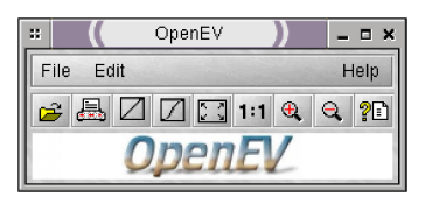
\includegraphics{toolbar.eps}
\caption{Basic Icon Bar}
\label{fig:iconbar}
\end{figure}

\section{Layer Control}
\label{sec:layer-control}

The layer control dialog provides the user with a list of layers
associated with a view area, and provides some controls to manipulate
the layers, and the ability to launch layer-specific properties panels.  
Layer manipulation functions accessible via the layer control dialog, or
layer-specific properties panels include:

\begin{itemize}
\item Change the active (selected) layer.
\item Raise or lower a layer.
\item Delete a layer.
\item Change the name of a layer.
\item Change the visibility of a layer.
\item Change the opacity of a layer.
\item Change the default color of a layer.
\item Change the raster scaling parameters of a layer.
\item Change the raster interpolation schema for a layer.
\item Change the raster bands used for a layer.
\end{itemize}
Layers are identified by name, and by a thumbnail image.  Figure
\ref{fig:layerdlg} shows a conceptual layer dialog.

\begin{figure}
\centering
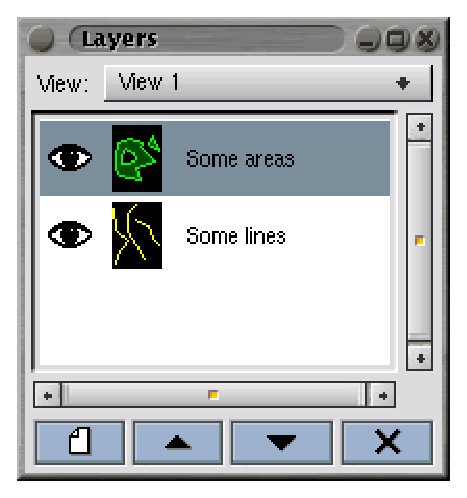
\includegraphics{layerdlg.eps}
\caption{Conceptual Layer Dialog}
\label{fig:layerdlg}
\end{figure}

\section{Toolbar}

The toolbar dialog is a simple button box widget connected to a OpenEV
toolbox tool.  The user changes the currently active tool with this
dialog.

\section{On-Line Help}
\label{sec:online-help}

A general on-line help system, based on HTML formatted help pages, is
available for OpenEV application development.  Providing access to help
is the responsibility of the application, but is normally provided in
a drop down menu.  Help pages are viewed through a user configurable
external web browser.

Applications use the python {\tt gvhtml.LaunchHTML()} to display help or
other web pages.  

\section{Printing}

In order to enable printing, the GvViewArea has the ability to render
its contents at an arbitrary resolution, providing the resulting raster 
RGB data to application callbacks.  Particular mechanisms are built on
this to write the result to PostScript, or any GDAL supported raster format.

The rendering mechanism is invoked by the 
{\tt gv\_view\_area\_render\_to\_func() }
function, which takes a view to render, a resolution and a callback to 
provide the data to. The rendering is accomplished by altering the view port
and rendering into the backbuffer of the GvViewArea.  This is fetched
by using the glReadPixels() call to fetch the result back from the
back buffer.  

One downside to this approach is that on eight or sixteen bit
display systems, the resulting rendering is normally done at the
color resolution of the visual.  Also, it appears some GL implementations
(such as the 1999 Linux NVidia drivers) don't support glReadPixels(). 
However, the greatest limitation with this architecture is that text, and
vector graphics are rendered at the same resolution as the raster data
rather than being transported in descriptive form to be rendered by the
printer at it's best resolution.  

For higher resolution renderings the region to render is split into smaller 
tiles matching the size of the viewport, and the result reassembled for
output.  

Currently output drivers exist for PostScript 
({\tt gv\_view\_area\_print\_postscript\_to\_file()}) and GDAL supported raster 
formats such as TIFF and PNG 
({\tt gv\_view\_area\_print\_to\_file()}).  In time it is expected to implement
support for a few other common outputs such as HPGL and writing directly to
MS Windows printer drivers. 


\begin{thebibliography}{9}

\bibitem{woo:opengl} M.Woo, J.Neider, T.Davis, D.Schreiner, OpenGL
Architecture Review Board, \emph{OpenGL Programming Guide: The
Official Guide to Learning OpenGL, Version 1.2}, 3rd ed.,
Addison-Wesley, 1999.

\bibitem{gtk.org} The GIMP Toolkit homepage.  http://www.gtk.org

\bibitem{mor:ogdi} P.Morin, \emph{OGDI: Programmer Reference},
ver. 3.0, OGDI Research Institute, OGDI-RI-98001, May 1998.\\
http://132.156.30.81/iii/docs/programmers\_guide/ogdi.pdf

\end{thebibliography}

\end{document}
